\documentclass[a4paper,10pt]{article} 
\usepackage[utf8]{inputenc}
\usepackage[a4paper]{geometry}
\usepackage[magyar]{babel}
\usepackage{amsmath}
\usepackage{amssymb}
\usepackage{wrapfig}
\usepackage{pgf, tikz}
\frenchspacing 
\pagestyle{empty}
\newcommand{\ki}[2]{\hfill {\it #1 (#2)}\medskip}
\newcommand{\vonal}{\hbox to \hsize{\hskip2truecm\hrulefill\hskip2truecm}}
\newcommand{\degre}{\ensuremath{^\circ}}
\newcommand{\tg}{\mathop{\mathrm{tg}}\nolimits}
\newcommand{\ctg}{\mathop{\mathrm{ctg}}\nolimits}
\newcommand{\arc}{\mathop{\mathrm{arc}}\nolimits}
\begin{document}
\begin{center} \Large {\em 24. Nemzetközi Magyar Matematika Verseny} \end{center}
\begin{center} \large{\em Szabadka, 2015. április 8-12.} \end{center}
\smallskip
\begin{center} \large{\bf 9. osztály} \end{center}
\bigskip 

{\bf 1. feladat: } Egy
$20 \times 20$-as négyzetháló négyzeteibe a bal
felső mezőből indulva soronként  
sorra beírjuk az
$1, 2, 3,\ldots , 400$
pozitív egész számokat.
Ezután a
táblázat négyzeteiből az ábrán látható kereszt
alakú síkidommal mindig ötöt letakarunk az összes
lehetséges módon.\\
\centerline{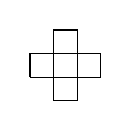
\begin{tikzpicture}[x=0.3cm,y=0.3cm]
\clip (-0.1,-0.1) rectangle (3.1,3.1);
\draw (1,0)--(2,0)--(2,3)--(1,3)--(1,0);
\draw (0,1)--(3,1)--(3,2)--(0,2)--(0,1);
\end{tikzpicture}}\\
Hányszor lesz a letakart öt szám
összege négyzetszám? Milyen szám áll ezekben az
esetekben a kereszt közepén?

\ki{Nemecskó István}{Budapest, Magyarország}\medskip

{\bf 2. feladat: } Egy háromjegyű számot osztva a számjegyeinek összegével $37$-et kapunk. Ha e
háromjegyű számhoz hozzáadunk $297$-et, a megfordított (felcserélt sorrendben
felírt) számjegyek\-ből álló számot kapjuk. Mely háromjegyű számok esetében
lehetséges ez?

\ki{Kovács Béla}{Szatmárnémeti, Erdély}\medskip

{\bf 3. feladat: } Hány megoldása van a prímszámok halmazában a
$p^2 + q^2 + r^2 + s^2 = pqrs + 4$
egyenletnek?

\ki{Mészáros József}{Galánta, Felvidék}\medskip

{\bf 4. feladat: } Egy $ABC$
háromszögben
$A \sphericalangle = 60^\circ$. 
Legyenek rendre az $M$ és $N$
pontok az $AB$ és $AC$
oldalak olyan pontjai, melyekre
$AM = CN$. 
Az $MN$ szakasz felezőpontja legyen $F_1$, míg az $AC$
oldal felezőpontja $F_2$. Bizonyítsd be, hogy
$$F_1F_2 = \frac{1}{2}\cdot AM. $$

\ki{Bíró Béla}{Sepsiszentgyörgy, Erdély}\medskip

{\bf 5. feladat: } Keresd meg az összes olyan pozitív egészekből álló
 $(x , y , z)$ 
számhármast,
amelyre érvényes, hogy
$ x \mid (y + 1),\quad 2y \mid (z+2) \quad
\text{~és~}\quad
3z \mid (x + 3)$.

\ki{Kekeňak Szilvia}{Kassa, Felvidék}\medskip

{\bf 6. feladat: }  Az $ABC$
hegyesszögű háromszög magasságpontja $M$. 
Igazold, hogy ha $MC = AB$, akkor az
$ACB\sphericalangle=45^\circ$. 
Igaz-e az állítás tompaszögű háromszögben is?


\ki{Katz Sándor}{Bonyhád, Magyarország}\medskip


\end{document}